\section{Results}
\label{sec:results}

All values are means over seeds with the seed count stated, with BCa 95\%
intervals; per-seed raw results ship with the artifact. \macroF{} on the
pooled global test set under the realistic class prior is the headline
metric. The section leads with the reference frame under the
leakage-controlled chronological split -- the headline protocol -- then
reads the pre-registered random split as a leakage-inflated diagnostic
ceiling, then reports the pre-registered hypotheses, several of which did
not survive their own decision rules.

\subsection{Reference frame under the leakage-controlled split}
\label{sec:res-frame}

The two protocols bracket every absolute number, and differ in whether a
test window may share samples with a training one: windows are cut at
stride~16 over length~64 ($75\%$ overlap), and the committed measurement
script finds $99.9\%$ of test windows overlapping a training window under
the random split against $\approx 0\%$ under the chronological one.
Figure~\ref{fig:temporal_frame} puts both protocols side by side for the
full frame (exact cells: Table~\ref{tab:temporal_frame}).

\begin{figure}[tbp]
\centering
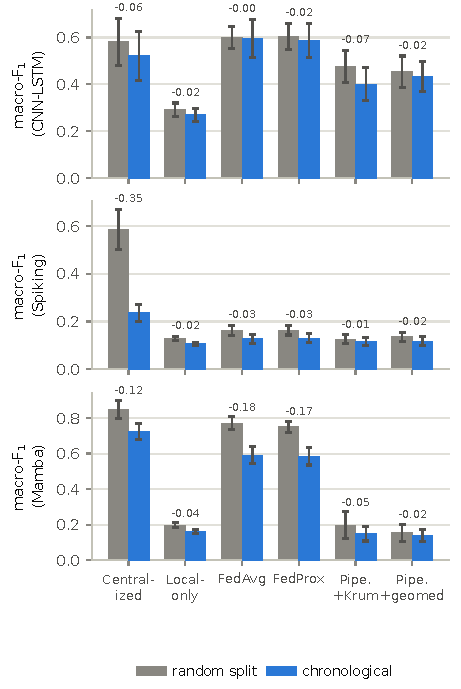
\includegraphics[width=\linewidth]{figures/fig_split_frame}
\caption{Reference-frame \macroF{} (mean $\pm$ sd) per arm and model, chronological split (T1a\_temporal) beside random split (T1a), 15 seeds; numbers give the unpaired change. Cells: Table~\ref{tab:temporal_frame}.}
\label{fig:temporal_frame}
\end{figure}

\paragraph{The margin was leakage: the two dense models tie}
The ranking survives as a tie at the top, not a lead. Under FedAvg the
CNN-LSTM and the state-space model land on each other -- \macroF{}
$0.596$ against $0.590$, a paired difference an exact two-sided Wilcoxon
cannot separate ($p=0.56$) -- and the spiking model sits at $0.128$;
FedProx repeats the shape ($0.587/0.585/0.130$). Most arms lose
$5$--$25\%$ of their random-split score and the floor moves with
everything else; the spiking ceiling loses more (below). The exception
is the federated CNN-LSTM, statistically indifferent to the split
(FedAvg $-0.6\%$, $p=0.89$; FedProx $-2.7\%$): the random
protocol was crediting leakage accuracy to the state-space and spiking
arms and to both bounds, not to the reference. What changes is the claim
-- the state-space model's earlier lead was a margin on leaky cells.

\paragraph{The spiking ceiling was mostly leakage}
The largest single change is not in a federated row: the centralized
spiking ceiling falls $0.586 \rightarrow 0.236$ ($-60\%$) against
$-10\%$/$-15\%$ for the dense ceilings, on matched recipes. The model is
on the floor in \emph{both} regimes ($0.236$ centralized, $0.128$
federated, $0.121$ trivial predictor) -- not a structural limit of
\emph{federated} surrogate-gradient training but the blunter finding
that this architecture does not learn this task at this budget. The
ceiling bounds only two of three arms, too: pooling the CNN-LSTM does
not beat its federated arm ($0.522$ vs.\ $0.596$ chronological, n.s.),
the per-client effective-number reweighting \cite{cui2019} being
miscalibrated on the pooled corpus.

\paragraph{A shallow probe, and the channel it audits}
A deep model is only justified if a cheap one cannot do the job. A
gradient-boosted tree at library defaults reaches \macroF{} $0.692$
pooled and $0.533$ under the chronological cut -- at or above the
CNN-LSTM's \emph{centralized} ceiling under either protocol, so the
reference is justified by timing (Section~\ref{sec:res-latency}), not
centralized accuracy; only its \emph{federated} arm ($0.596$) edges the
pooled probe ($0.692$ leans on default early stopping -- disabled,
$0.275$; detail in Section~\ref{sec:sup-probe}). The same probe audits
the sharpest benchmark shortcut: dropping the synthetic
$f_{\mathrm{dev}}$ channel costs $-0.011$/$-0.027$ \macroF{}
(random/temporal, intervals spanning zero) while the channel alone
reaches $0.295$/$0.234$ -- real but far-from-sufficient signal
(Table~\ref{tab:fdev}). Convergence is in Figure~\ref{fig:rounds}: only
the CNN-LSTM averaging arms reach their ceiling, on every seed.

\subsection{The random split as a leakage-inflated diagnostic}
\label{sec:res-temporal}

What the random split was crediting is visible cell by cell in
Figure~\ref{fig:temporal_attack}: cells carrying real accuracy give up as
much as $0.19$; the pipeline cells barely move, because the random split
only credits accuracy to arms that had accuracy to inflate. The two
results the defense analysis rests on both reproduce under the
controlled protocol: geomed-alone still recovers the loud attacks
(Gaussian noise on the CNN-LSTM: $0.059 \rightarrow 0.541$), and the
full pipeline is still catastrophic against the defense-aware attacker
(pipeline+Krum holds Mamba at $0.051$ where no defense holds $0.553$).
One confound comes with the cut: the test slice moves to a year-end
segment, so every $\Delta$ mixes leakage removal with seasonal shift --
the \emph{differential} pattern argues the leakage term dominates. Both
protocols therefore stay: the random-split battery
(Tables~\ref{tab:frame} and~\ref{tab:attackdefense}) carries the sweeps
and the pre-registered verdicts, and the temporal columns are the ones
to quote for absolute accuracy.

\begin{figure}[tbp]
\centering
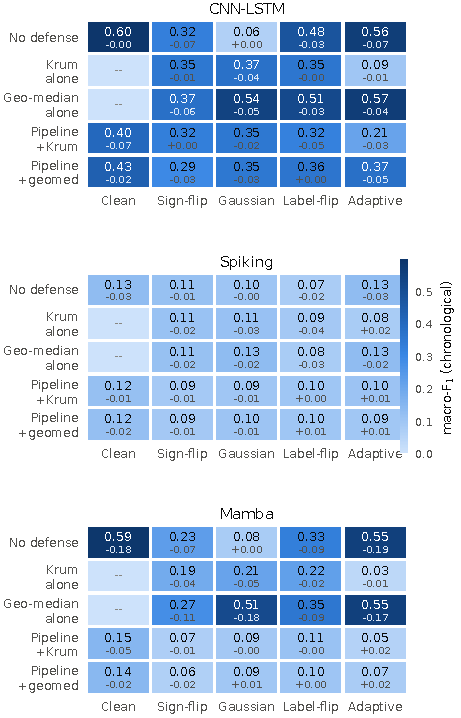
\includegraphics[width=\linewidth]{figures/fig_attack_heatmap}
\caption{Attack $\times$ defense \macroF{}, chronological split (T1b\_temporal, $f_{\mathrm{att}}=3/10$, 15 seeds), one panel per model; second line: change against the random split. Cells: Table~\ref{tab:temporal_attack}.}
\label{fig:temporal_attack}
\end{figure}

\subsection{H1: accuracy parity and the energy ratio}
\label{sec:res-energy}

\begin{figure}[tbp]
\centering
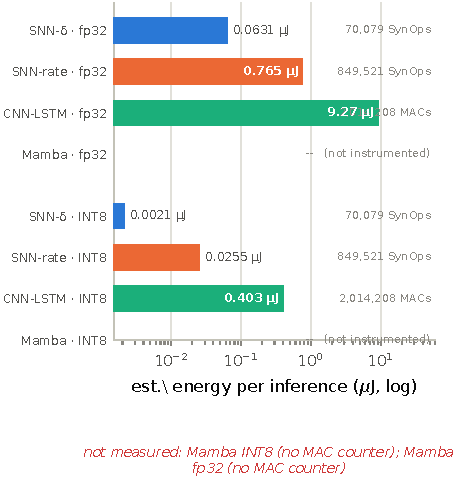
\includegraphics[width=\linewidth]{figures/fig_energy_bars}
\caption{Estimated energy per inference (log scale) per model and coding at $T{=}8$, 45\,nm constants \cite{horowitz2014}. Arithmetic-only SynOps estimate, not a hardware measurement. Cells: Table~\ref{tab:energy}.}
\label{fig:energy}
\end{figure}

The pre-registered parity claim fails decisively: McNemar's exact test
rejects equality ($p<0.001$) and the paired $\Delta$\macroF{} lies far
outside the $\pm0.02$ equivalence margin (BCa 95\% $[-0.465,-0.417]$).
What survives is the energy accounting (Figure~\ref{fig:energy}): under
delta coding the spiking model performs $70\,079$ synaptic operations
per inference against $2\,014\,208$ multiply--accumulates -- an
estimated $0.063$ against $9.27$ microjoules, a ratio $\rho \approx
6.8\times10^{-3}$ with the one-sided BCa interval wholly below one: H1b
is supported, H1a is not, and H1 fails as a conjunction. Rate coding
costs an order of magnitude more for less accuracy
(Section~\ref{sec:res-ablations}); Mamba reads $21.1$\,\uJ{},
$2.3\times$ the reference. These are arithmetic-only estimates, not
hardware measurements. The spiking model delivers its energy reduction
only by conceding almost all of its federated accuracy --
Figure~\ref{fig:energyacc} places every costed arm on the
accuracy--energy plane.

\subsection{Latency against the fast-message envelope}
\label{sec:res-latency}

Inference is one term of the end-to-end chain, so a measured p99 is a
\emph{compute share} of a co-resident 4\,ms fast-message envelope, not a
compliance verdict on it (Figure~\ref{fig:latencyenv}). At fp32 only the
CNN-LSTM leaves any of
the envelope, and only on GPU: $3.28$\,ms p99, $82\%$ of it, against
$212\%$ on CPU; the spiking model ($402$--$423\%$) and Mamba
($548$--$615\%$) exceed the whole envelope alone, and no model benefits
from dynamic INT8 quantization -- torch's kernels reject the recurrent
and state-space packed parameters, so every measured latency is fp32
(distributions in Supplementary Figure~\ref{fig:latency}). The three
architectures resolve into a clean trade-off: Mamba ties for the
accuracy lead but is slowest, the spiking model is cheapest but neither
accurate nor fast, and the reference is the only one whose compute would
fit beside a protection-adjacent function -- on one fixed reference
machine, which orders the models but certifies no substation device.

\begin{figure}[tbp]
\centering
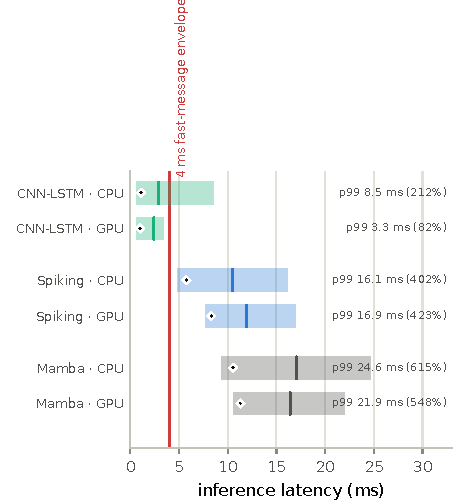
\includegraphics[width=\linewidth]{figures/fig_latency_env}
\caption{Measured inference latency (fp32, batch 1, $n=1000$) per model and device against the 4\,ms fast-message envelope; bar p50--p99, tick p95, diamond mean. A compute share, not compliance. Cells: Table~\ref{tab:latency}.}
\label{fig:latencyenv}
\end{figure}

\subsection{H2: the pipeline under attack}
\label{sec:res-attack}

The grid does not reward the pipeline; this is the paper's central
negative result (Table~\ref{tab:attackdefense}, decomposed rung by rung
in Table~\ref{tab:decomp}). Under the defense-aware attacker,
geometric-median aggregation \emph{alone} preserves accuracy almost
perfectly (CNN-LSTM $-0.020$ from no defense; Mamba $-0.013$) while
rejecting nobody, whereas the same aggregator behind the gate and PBFT
drops to $0.420$/$0.051$ and rejects $66$--$97\%$ of honest updates.
Krum alone is worse than useless -- the single-update selector is
exactly what the cosine-aligned attacker games ($0.043$--$0.100$) -- and
the pipeline compounds the damage: Krum's guarantee needs
$n \ge 2f+3 = 9$ admitted updates at $f=3$, and a gate rejecting most of
the honest population routinely hands it fewer. Under the loud attacks a
robust aggregator recovers most of the loss, the gate never adds
accuracy over the bare aggregator, and Mamba under the adaptive attack
with \emph{no} defense holds $0.739$: it is robust by itself, and the
pipeline takes that away.

The Friedman test agrees under both blockings (Figure~\ref{fig:cd}): at
the pre-registered blocking exactly two pairs separate --
geometric-median-alone above each pipeline arm -- and no-defense against
pipeline+Krum does \emph{not}. Two of the $24$ per-cell tests support
the pipeline after Holm correction (both aggregators against Gaussian
noise on the CNN-LSTM, $\delta=+1.00$) -- loud attacks on the weaker
model, not the defense-aware attacker the pipeline was built for
(Table~\ref{tab:stats}). H2 is recorded as not supported
(Table~\ref{tab:hypotheses}), with the qualification that the agreement
layer contributes the audit record and the measured overhead, not
accuracy; the attack-fraction sweep (T2b) moves the same way.

\subsection{Opening the gate: the admission-threshold sweep}
\label{sec:res-tau}

The pre-registered $\tau=0.5$ is one point on a curve, and sweeping it
changes the diagnosis (Table~\ref{tab:tau_sweep}). As $\tau$ opens to
$1.0$ the gate stops rejecting honest clients (FRR $0.68$--$0.97
\rightarrow \le 0.016$) while the defense-aware attacker is admitted
essentially always ($\ge 0.92$ at $\tau \ge 0.8$) -- the worst of both
worlds on the registered decision rule. What it produces is not: behind
the geometric median accuracy \emph{recovers} as the gate opens
($0.184 \rightarrow 0.487$ pooled; Mamba $0.051 \rightarrow 0.718$,
within $0.01$ of geo-median-alone), while behind Krum it collapses
further ($0.120 \rightarrow 0.069$). This revises H2 rather than
reversing it: at $\tau=0.5$ the gate was \emph{throttling its own
aggregator} -- the negative result is about calibration, not mechanism,
and no setting of $\tau$ makes the pipeline \emph{add} accuracy over the
bare aggregator.

\subsection{H3: the defense-aware attacker's evasion--damage asymmetry}
\label{sec:res-adaptive}

The mechanism behaves exactly as designed, and at fifteen seeds it gets
its statistical answer (Table~\ref{tab:adaptive}). Against either
aggregator the defense-aware attacker holds its realized score to
$0.40$--$0.55$, straddling $\tau=0.5$, where the loud sign-flip scores
$0.98$--$1.05$ and is rejected outright: admission rises from $0.000$ to
$0.53$--$0.59$ and to $0.87$ against Mamba, at
$p_{\mathrm{Holm}} = 1.8\times10^{-4}$ in all six cells -- the evasion is
real and H3a is supported. The same gate still rejects $66$--$98\%$ of
\emph{honest} updates: it does not separate friend from foe, it rejects
both. The damage leg splits by aggregator: behind Krum the admitted
attack costs \emph{more} than the rejected sign-flip on two of three
models ($0.242$ vs.\ $0.153$; $0.167$ vs.\ $0.122$, both significant);
behind the geometric median it runs backwards ($0.034$ vs.\ $0.134$),
because a robust average is not moved by an update it was content to
admit. H3b stays not supported on its $2/6$ cell count -- a property of
the averaging aggregator, not of the test's resolution.

\subsection{The attacker's magnitude lever}
\label{sec:res-magnitude}

\begin{figure}[tbp]
\centering
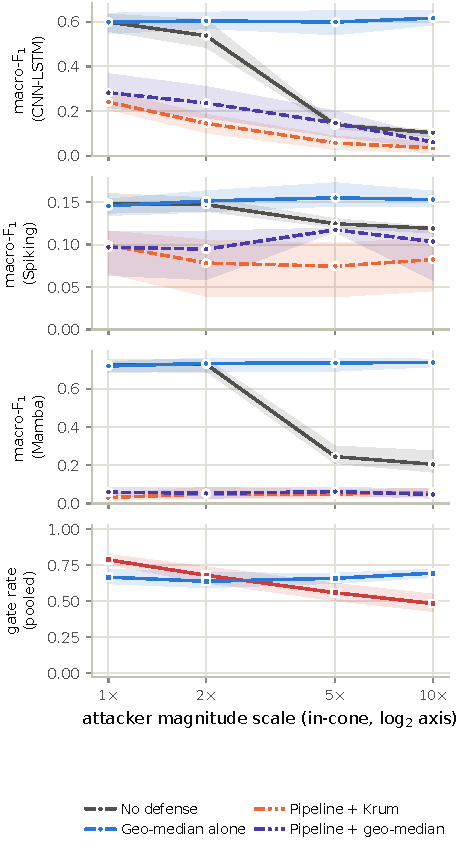
\includegraphics[width=\linewidth]{figures/fig_magnitude}
\caption{\macroF{} (BCa bands) and pooled gate rates as the in-cone attacker scales its update by $s\in\{1,2,5,10\}$ (T4mag, random split, $f_{\mathrm{att}}=3/10$, 9 seeds); $s{=}1$ is the default. Cells: Table~\ref{tab:magnitude}.}
\label{fig:magnitude}
\end{figure}

Cosine scoring is scale-free, so an in-cone attacker can multiply its
update without moving its fidelity score; the pre-registered battery
left that factor at $1$ throughout, and block T4mag sweeps it
(Figure~\ref{fig:magnitude}). Three things happen, and they point the
same way. \emph{Plain averaging breaks}: the undefended CNN-LSTM falls
$0.598 \rightarrow 0.103$ and Mamba $0.727 \rightarrow 0.205$ --
significant at $5\times$--$10\times$ on the dense models, descriptively
the damage leg H3b failed to find at unit magnitude. \emph{The geometric
median is invariant to the lever}: its cells move by at most $+0.019$, a
breakdown-point argument appearing as a measurement. \emph{The gate
loosens under the lever}: the attacker's score barely moves
($0.466 \rightarrow 0.417$) while honest false-rejection falls
$0.799 \rightarrow 0.476$ -- the honest population's own mean score
slides through the fixed threshold ($0.608 \rightarrow 0.470$),
collapsing the discriminative gap ($0.142 \rightarrow 0.052$). The gate
loosens not because the attacker climbs toward the threshold but because
the honest clients slide down through it; neither gated arm profits.

\subsection{H4: the privacy-versus-admission operating curve}
\label{sec:res-ldp}

\begin{figure}[tbp]
\centering
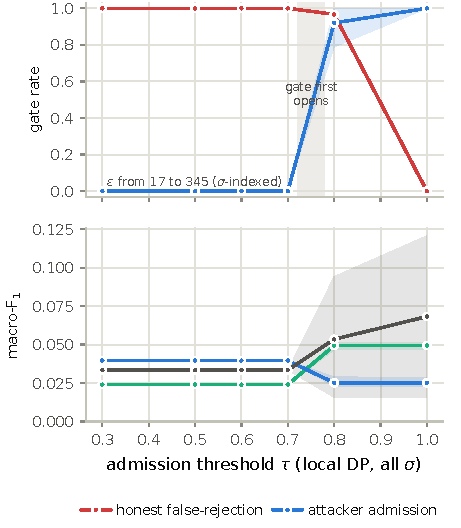
\includegraphics[width=\linewidth]{figures/fig_ldp_tau}
\caption{Gate rates (top) and \macroF{} (bottom) against $\tau$ on pipeline+Krum under the defense-aware attacker, pooled over four $\sigma$ (band: cross-$\sigma$ range; T2c and T3$\tau$, random split, 9 seeds). Cells: Table~\ref{tab:ldp_tau_extended}.}
\label{fig:ldp_tau}
\end{figure}

The operating curve is degenerate, and the extended sweep shows why
(Figure~\ref{fig:ldp_tau}). Across all twelve registered
$(\sigma,\tau)$ points the honest false-rejection rate is pinned at
$1.000$ and the attacker admission reads $0.000$ only because
\emph{nothing} is admitted -- the gate rejects all ten clients in all
thirty rounds, the model never leaves initialization, and the reported
\macroF{} is an untrained network's, below even the $0.121$ majority
floor; the ordered-trend test is correspondingly flat
(Jonckheere--Terpstra $p=0.500$), so H4 is not supported. The gate first
opens between $\tau=0.7$ and $0.8$; past it the attacker is admitted
$0.788$--$1.000$ and \macroF{} stays on the floor: no corner that was
run buys the accuracy back (two caveats: the extension is pipeline+Krum
only, and six runs diverged on non-finite scores -- excluded, ``div.'').
The argument is dimensional, not a tuning failure: on $\sim
10^{5}$-parameter updates, isotropic noise calibrated for local DP must
overwhelm the update direction entirely -- the scored cosine becomes
noise -- and even the weakest setting carries a near-vacuous budget
($\varepsilon$ from $16.9$ to $345$). Update-level local DP and cosine
admission are, on this architecture, mutually exclusive: a
near-impossibility we quantify rather than a curve we tune.

\subsection{H5: heterogeneity}
\label{sec:res-alpha}

Heterogeneity degrades the two weaker models and leaves the state-space
model alone -- not the pre-registered prediction
(Table~\ref{tab:alpha}). From the near-uniform control to
$\alpha = 0.1$, FedAvg CNN-LSTM \macroF{} falls $0.683 \rightarrow
0.499$ and FedAvg spiking $0.190 \rightarrow 0.118$, while FedAvg Mamba
does not move outside seed noise ($0.770 \rightarrow 0.798$, in the
wrong direction). Four of six ordered-trend tests survive Holm
correction -- both weaker models on both arms -- while both Mamba trends
stay flat at $n=42$ runs per trend, so H5a fails its decision rule on
architecture, not power. H5b fails too: exactly one of three cells
clears the floor (spiking, $\delta=+0.88$), the CNN-LSTM cell inverts
($\delta=-0.51$) and Mamba's is flat. The conjunction fails on both legs
for two different reasons; the state-space model is simply insensitive
to label skew over the swept range -- a finding, not a failure.

\subsection{Consensus overhead}
\label{sec:res-consensus}

At the default committee a committing round costs exactly $180$ messages
and $167.8$\,ms of simulated wide-area latency against a training round
orders of magnitude longer, so agreement is not the bottleneck
(Table~\ref{tab:consensus}). The sweep's accuracy reading is no
robustness story: pipeline+Krum is already collapsed at every committee
size, and the moves between $M \in \{4,7,10\}$ are seed variance of a
collapsed arm -- overhead without accuracy return at this operating
point. And the auditability claim is bounded exactly: pipeline arms
append every round to a SHA-256 chain, but no \texttt{RunResult}
carries an end-to-end verification, so auditability is a design claim
with property-test coverage, not a measurement; the latency is a lower
bound (Section~\ref{sec:threat}).

\subsection{Per-class behaviour}
\label{sec:res-perclass}

\begin{figure}[tbp]
\centering
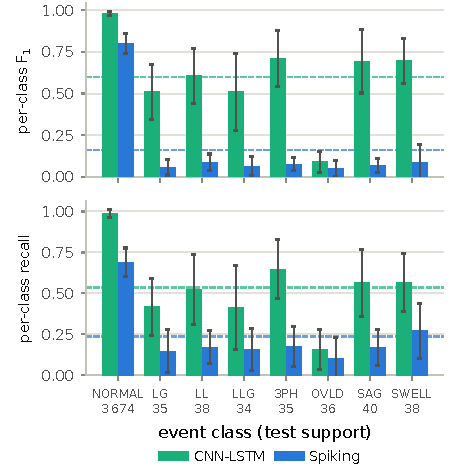
\includegraphics[width=\linewidth]{figures/fig_perclass}
\caption{Per-class F\textsubscript{1} and recall (mean $\pm$ sd; dashed: macro score) with mean test support, clean FedAvg reference (T1a, random split, 15 seeds). Cells: Table~\ref{tab:perclass}.}
\label{fig:perclass}
\end{figure}

The macro average hides a rare-event problem
(Figure~\ref{fig:perclass}). At the clean FedAvg reference the CNN-LSTM
carries \cls{normal} almost perfectly ($F_1 = 0.983$) but degrades on
the fault and power-quality classes whose support is in the tens -- down
to $F_1 = 0.089$ on \cls{overload} -- so its $0.600$ is a rare-class
average. The spiking model fails these outright: on \cls{fault\_lg} its
recall of $0.147$ comes with near-zero precision -- the collapsed model
sprays the rare label rather than never predicting it. These are
statements about class rarity, not intrinsic detectability.

\subsection{Ablations and the real-trace sanity check}
\label{sec:res-ablations}
\label{sec:res-real}

Neither ablation rescues the spiking collapse or improves on FedAvg
(Tables~\ref{tab:coding} and~\ref{tab:fedprox}). Under delta coding,
shortening the unroll helps -- $T=4$ gives the best clean \macroF{} at
$0.204$ against $T=8$'s $0.161$ -- so longer integration buys more
SynOps for \emph{less} accuracy, and rate coding pins at the trivial
floor; the most favourable spiking configuration sits at about a quarter
of Mamba's federated \macroF{}. FedProx is inert (largest paired gain
$+0.006$; Mamba at $\mu=0.1$ loses $0.150$). On the MSU/ORNL real
traces -- a sanity check read narrowly: near-IID, effectively binary,
random split, $n=3$ -- every arm runs to completion and the ordering
\emph{inverts} (spiking $0.996$, Mamba $1.000$, CNN-LSTM $0.703$;
pipeline $0.927$--$0.990$ on the spiking and Mamba models,
$0.486$--$0.726$ on the CNN-LSTM): the pipeline is operable on real
IEC~61850-adjacent traces, but the set does not validate the synthetic
benchmark.

\subsection{Statistical battery and hypothesis verdicts}
\label{sec:res-stats}

Table~\ref{tab:stats} collects the complete battery and
Table~\ref{tab:hypotheses} the verdicts, and the scoreboard is
unflattering but fully decidable: exactly two hypotheses are supported
-- H1b (the spiking energy ratio below one) and H3a (the defense-aware
evasion) -- while H1a, H2, H3b, H4, H5a and H5b are not, and the
conjunctions fail with them; none is a power artefact any more. What the
tables do support is an open, honestly scored benchmark carrying four
durable findings: a three-corner model trade-off whose accuracy corner
is \emph{shared} between the two dense models; a negative result on
elaborate Byzantine admission -- robust averaging alone suffices and the
gate buys auditability, not accuracy; an unpredicted heterogeneity
result -- the co-leading architecture is indifferent to label skew; and
the one attack that breaks plain averaging -- in-cone magnitude --
against which the geometric median is invariant and the gate loosens.
